\subsection{Part Selection}
\subsubsection{Controller Subsystem}
\begin{flushleft}
	At minimum, any chosen microcontrollers (MCUs) shall support natively, or by addition of a
	module, these features and traits:
	\begin{itemize}
		\item Analog-to-digital converter (ADC)
		\item cURL compatibility
		\item IEEE 802.11
		\item In stock and available to order
		\item JTAG module or equivalent
		\item Module communication bus (UART, I2C, SPI)
		\item Onboard CPU sufficient for our purposes
		\item Onboard memory sufficient for our purposes
		\item Onboard nonvolatile memory
		\item Pins dedicated to analog input
		\item Pins dedicated to digital I/O
	\end{itemize}
	These features would be "nice to have" on any MCU selected, but are not required:
	\begin{itemize}
		\item Digital-to-analog converter (DAC)
		\item microSD card slot
		\item Onboard battery
		\item Pins dedicated to pulse-width modulation (PWM)
		\item Timer(s) and an RTC
		\item USB compatibility
		\item Additional wireless communication protocols (e.g. BT or BLE, Zigbee)
	\end{itemize}
\end{flushleft}
\begin{flushleft}
	The selections, listed in \autoref{table:mcubreakdown1} and not in any particular order, match
	the above criteria and are being considered for selection.
	\begin{table}
		\centering
		\begin{tabularx}{\textwidth}
			{
				| >{\raggedright\arraybackslash}X
				| >{\raggedright\arraybackslash}X
				| >{\raggedright\arraybackslash}X
				| >{\raggedright\arraybackslash}X
				| >{\raggedright\arraybackslash}X
				| >{\raggedright\arraybackslash}X
				|
			}
			\caption{MCU option breakdown}
			\label{table:mcubreakdown1} \\
			\hline
			\textbf{Model} & \textbf{\href{https://www.ti.com/tool/LAUNCHXL-CC26X2R1}{LAUNCH\-XL-CC26X2\-R1}} & \textbf{\href{https://www.ti.com/tool/LAUNCHCC3220MODASF}{LAUNCH\-CC3220\-MODASF}} & \textbf{\href{https://www.raspberrypi.com/products/raspberry-pi-pico/}{Pico W}} & \textbf{\href{https://store-usa.arduino.cc/products/arduino-nano-33-ble?selectedStore=u}{Nano 33 BLE}} & \textbf{\href{https://www.st.com/en/evaluation-tools/b-l4s5i-iot01a.html}{B-L4S5I-IOT01A}} \\
			\hline
			\textbf{Manu\-facturer} & Texas Instruments & Texas Instruments & Raspberry Pi & Arduino & STMicro\-electronics \\
			\hline
			\textbf{Micro\-controller} & CC2652R & CC3220\-MODASF & RP2040 & nRF52840 & STM32\-L4S5VIT6 \\
			\hline
			\textbf{Processor} & 1x ARM Cortex-M4F & 1x ARM Cortex-M4 & 2x ARM Cortex-M0+ & 1x ARM Cortex-M4 & 1x ARM Cortex-M4 \\
			\hline
			\textbf{Maximum Speed (MHz)} & 48 & 80 & 133 & 64 & 120 \\
			\hline
			\textbf{Memory (KB)} & 256 ROM, 352 flash, 100 SRAM & 1024 flash, 256 RAM & 16 ROM, 264 SRAM & 1024 flash, 256 SRAM & 2048 flash, 640 RAM \\
			\hline
			\textbf{Wireless capability} & BLE5.2, Zigbee, Thread & 802.11b/g/n & 802.11n & BLE5.3, Zigbee, Thread, Matter & BT4.1, 802.11b/g/n, NFC \\
			\hline
			\textbf{Serial capability} & UART, I2C, I2S, SPI & UART, I2C, SPI & UART, I2C, SPI, USB1.1 & UART, I2C, I2S, SPI, USB2.0 & UART, I2C, SPI, USB2.0 \\
			\hline
			\textbf{Price (\$)} & 40, maybe free & 60, maybe free & 6 & 28 & 53 \\
			\hline
			\textbf{ADC} & 8-channel, 12-bit & 4-channel, 12-bit & 4-channel, 12-bit & 8-channel, 12-bit & 16-channel, 12-bit \\
			\hline
			\textbf{Clock capability} & Timer, RTC & Timer, RTC, WDT & Timer, RTC, WDT & Timer, RTC, WDT & Timer, RTC, WDT \\
			\hline
			\textbf{GPIO (pins)} & 31 & 29 & 30 & 13 & 16 \\
			\hline
			\textbf{PWM (channels)} & Supported & Supported & 16 & 4 & 6 \\
			\hline
			% \textbf{AES (bits)} & 128, 256 & 256 & Not supported & 128 & 128 \\
			% \hline
			\textbf{Required voltage (V)} & 1.8 -- 3.8 & 2.3 -- 3.6 & 1.8 -- 3.3 & 4.5 -- 21 & 4.75 -- 5.25 \\
			\hline
		\end{tabularx}
	\end{table}
\end{flushleft}
\begin{flushleft}
	Use of single-board computers (SBCs) was considered, but will not not need to be used; cURL 
	used on an MCU in conjunction with \href{https://aws.amazon.com/ec2/}{Amazon EC2} services will
	allow us to offload computing to a cloud solution.
\end{flushleft}
\begin{flushleft}
	Use of an external Wifi module is discouraged due to the following:
	\begin{itemize}
		\item Added cost
		\item Added complexity
		\item Modules in common use by hobbyists often have poor or no proper documentation, to the
		extent of:
		\begin{itemize}
			\item Quick start guide
			\item User's guide
			\item Datasheets
			\item Theory of operation
			\item Application uses
			\item Troubleshooting guide
			\item Schematics and mechanicals
			\item Quality and reliability
			\item Errata
		\end{itemize}
	\end{itemize}
\end{flushleft}
\begin{flushleft}
	Therefore, all of the MCUs listed above support either the 802.11 or Bluetooth standards.
\end{flushleft}
\begin{flushleft}
	Ultimately, the \href{https://www.ti.com/tool/LAUNCHCC3220MODASF}{LAUNCHCC3220MODASF}
	was chosen as the microcontroller development board for this project. In the event that the
	aforementioned LaunchPad is not able to be obtained, the
	\href{https://www.ti.com/tool/CC3220SF-LAUNCHXL}{CC3220SF-LAUNCHXL} has equivalent capability
	for the project's needs.
\end{flushleft}
\begin{flushleft}
	These boards, henceforth referred to as the CC3220, are able to be requested from our
	university at no upfront cost to our team. This was the driving factor behind choosing 
	the CC3220 over other microcontroller development boards. It was also determined that
	the microcontroller \emph{must} be able to interface via the 802.11 (WiFi) standard, for reasons
	that are detailed in \autoref{sec:controller_subsystem}---therefore, the LAUNCHXL-CC26X2R1
	and Nano 33 BLE were disqualified from selection. The Pico W was considered due to its low cost,
	and the B-L4S5I-IOT01A considered because of its abundant peripherals, but both ultimately lost
	out to the Texas Instruments products.
\end{flushleft}
% End Controller Subsystem

\subsubsection{Power Subsystem}
At minimum, this power subsystem will operate with the following:
\begin{itemize}
	\item Solar Panels 
	\item Rechargeable Batteries 
	\item Solar Charge Controllers
	\item AC/DC converterter
\end{itemize}
\textbf{Solar Panels}\par
The stretch goal for this project is to use solar panel arrays as blinds to increase/decrease sunlight as well as temperature. The solar panels are also use tocollect energy and power our model. We must be strategic when choosing our solar panels so that they are operational, provide the proper amount of power, and more.\par
There are many different types of solar panels. These include monocrystalline solar panels, polycrystalline solar panels, and thin-film solar panels. Each solarpanel has different compositions that make it as efficient as they are, how much power can be collected, etc. \par
For this project, we have selected multiple types of solar panels based on efficiency and cost.
\begin{table}[H]
    \centering
	
	\begin{tabularx}{\textwidth}
		{
			| >{\raggedright\arraybackslash}X
			| >{\raggedright\arraybackslash}X
			| >{\raggedright\arraybackslash}X
			| >{\raggedright\arraybackslash}X
			|
		}
		\caption{Solar panel types}
		\label{table:solarpanel} \\
		\hline
		\textbf{Solar Panel Type} & \textbf{Mono\-crystalline} & \textbf{Poly\-crystalline} & \textbf{Thin - Film} \\
		\hline
		\textbf{Efficiency} &  \textgreater20\% & 15 - 17\% & 6 - 15\% \\
		\hline
		\textbf{Power Rating} &  $\le$300W & 240 - 300W & Indefinite \\
		\hline
		\textbf{Performance} & Most efficient & Efficient & Least efficient \\
		\hline
		\textbf{Temperature} & High Tolerance & Low Tolerance & High Tolerance \\
		\hline
		\textbf{Cost per Watt} & \$1 - \$1.50 & \$.70 - \$1 & \$.43 - \$.70 \\
		\hline
	\end{tabularx}
\end{table}
From there we found these solar panels:
\begin{table}[H]
    \centering
	\caption{Solar panel part breakdown}
	\label{table:solarpanelparts}
	\begin{tabularx}{\textwidth}
		{
			| >{\raggedright\arraybackslash}X
			| >{\raggedright\arraybackslash}X
			| >{\raggedright\arraybackslash}X
			| >{\raggedright\arraybackslash}X
			| >{\raggedright\arraybackslash}X
			| >{\raggedright\arraybackslash}X
			|
		}
		\hline
		\textbf{Manu\-facturer Part \#} & P108 & P103C & P105 & SP-80X60-4-DK & SP-68X37-4-DK \\
		\hline
		\textbf{Manu\-facturer} & Voltaic Systems & Voltaic Systems & Voltaic Systems & AMX Solar & AMX Solar \\
		\hline
		\textbf{Dim\-ensions} & 10.9 x 8.8 x .16 & 8.27 x 4.46 x .2 & 5.39 x 8.74 x 0.16 & 3.15 x 2.362 x .079 & 2.677  x 1.456  x 0.079 \\
		\hline
		\textbf{Voltage at Pmpp} & 17.34V & 6.5V & 6.12V & 1.5V & 5.28V \\ 
		\hline
		\textbf{Current at Pmpp} & 570mA & 550mA & 940mA & 440mA & 69.3mA \\
		\hline
		\textbf{Open Circuit Voltage} & 20.45V & 7.7V & 7.13V & 1.8V & 6.27V \\
		\hline
		\textbf{Price (\$)} & 49 & 39 & 35 & 36.65 & 28.94 \\
		\hline
	\end{tabularx}
\end{table}
From there we needed to choose what kind of rechargeable battery we wanted to use for. Out on the market there are many different types of batteries including Nickel-Cadmium(NiCd), Nickel-Metal Hydride(NiMH), Lithium Ion(Li-Ion), and so many more.\par
Of these batteries, we decided to go with the Lithium Ion battery because it was the most commonly used battery for electronic devices while allowing high output voltage.
\begin{table}[H]
    \centering
	\begin{tabularx}{\textwidth}
			{
			| >{\raggedright\arraybackslash}X
			| >{\raggedright\arraybackslash}X
			| >{\raggedright\arraybackslash}X
			| >{\raggedright\arraybackslash}X
			| >{\raggedright\arraybackslash}X
			|
		}
		\caption{Battery investigation}
		\label{table:battery} \\
		\hline
		\textbf{Manu\-facturer} & \textbf{Ampere Time} & \textbf{Expert\-Power} & \textbf{Eco Worthy} & \textbf{Eco Worthy} \\
		\hline
		\textbf{Voltage} & 12 & 12 & 12 & 12 \\
		\hline
		\textbf{mAh} & 6000 & 10000 & 5000 & 8000 \\
		\hline
		\textbf{Price (\$)} & 29.99 & 59.99 & 35.99 & 43.99 \\ 
		\hline
	\end{tabularx}
\end{table}
For the solar panels, having a solar charge controller is important to the system. The purpose of the solar charge controller is to optimize the charging of the battierys by the solar panels. There are two major types of solar charge controllers: Maximum Power Point Tracking (MPPT) and Pulse Width Modulated (PWM). \par 
With these two in mind we chose these charge conrollers:
\begin{table}[H]
    \centering
	\begin{tabularx}{\textwidth}
			{
			| >{\raggedright\arraybackslash}X
			| >{\raggedright\arraybackslash}X
			| >{\raggedright\arraybackslash}X
			| >{\raggedright\arraybackslash}X
			| >{\raggedright\arraybackslash}X
			|
		}
		\caption{Charge Controller}
		\label{table:chargecontroller} \\
		\hline
		\textbf{Manu\-facturer} & \textbf{Expert\-Power} & \textbf{Expert\-Power} & \textbf{Renogy} &  \textbf{Renogy} \\
		\hline
		\textbf{Nominal Voltage} & 12\slash24V  & 12\slash24V & 12\slash24V & 12\slash24V \\
		\hline
		\textbf{Rated Charge Current} & 10A & 20A & 10A & 30A \\
		\hline
		\textbf{Max PV Input Voltage} & 50V & 100V & 50V & 50V \\
		\hline
		\textbf{Self Consumption} & $\leq$10mA & $\leq$10mA & \textless10mA & $\leq$13mA \\
		\hline
		\textbf{Price (\$)} & 23.99 & 69.99 & 34.99 & 69.99 \\ 
		\hline
	\end{tabularx}
\end{table}


While the model is charging during the day or as a back up, this will be plugged into a wall outlet for power. This means we have to be able to convert the AC voltage coming from the wall is converted to DC voltage for the model to use.


\begin{table}[H]
    \centering
	\begin{tabularx}{.8\textwidth}
		{
			| >{\raggedright\arraybackslash}X
			| >{\raggedright\arraybackslash}X
			| >{\raggedright\arraybackslash}X
			| >{\raggedright\arraybackslash}X
			|
		}
		\caption{AC/DC Converter breakdown}
		\label{table:acdcconverter} \\
		\hline
		\textbf{Manu\-facturer} & \textbf{SmoTecQ} & \textbf{ANLINK} & \textbf{TMEZON} \\
		\hline
		\textbf{Input Voltage} &  240V & 100 - 240V & 100 - 240V \\
		\hline
		\textbf{Output Voltage} & 12V & 12V & 12V \\
		\hline
		\textbf{Current Rating} & 2A & 2A & 2A \\
		\hline
		\textbf{Connector} &  5.5 mm x 2.1 mm &  5.5 mm x 2.1 mm &  5.5 mm x 2.1 mm\\
		\hline
		\textbf{Price (\$)} & 12.99 for 2 & 11.59 & 8.99 \\ 
		\hline
	\end{tabularx}
\end{table}

\subsubsection{Sensing Subsystem}
The required sensing subsystem capabilities include:
    \begin{itemize}
        \item Spectral frequency separation
        \item Spectral range from 400 to 1700nm
        \item High Signal to Noise Ratio
    \end{itemize}


	Silicon photodiodes have a spectral range across the visible spectrum, usually spanning from 350 to 1000nm. In order to generate spectrographs with the relevant molecular fingerprints of soil substances, we're going to need an infrared detector. InGaAs stands out as the ideal material for this range, with most sensors ranging from 800 to 1700nm. There are several manufacturers of silicon photodiodes, and most of them offer a small selection of InGaAs photodiodes at low prices as well. Below are the four of each.


\begin{table}[H]
	\centering
	\label{table:VISsensors}
	\caption{VIS Sensors}
	\begin{tabular}{|p{2cm}|l|l|l|l|}
	\hline    
	Model & BPX 61 & ODD-5W & FDS100 & PIN-3CD\\
    \hline
	Manufacturer & Newark & Digikey Opto Diode Corp & Thorlabs & Edmund Optics\\
    \hline
	Spectral Range (nm) & 400-1100 & 300-1100 & 350-1100 & 350-1100\\
    \hline
	Active Area (mm sqrd) & 7.02 & 5 & 13 & 3.2\\
    \hline
	Cost (\$) & 13.06 & 14.50 & 16.08 & 34.00\\
    \hline
	\end{tabular}
\end{table}



\begin{table}[H]
	\centering
	\label{table:NIRsensors}
	\caption{NIR Sensors}
	\begin{tabular}{|p{2cm}|l|l|l|l|}
	\hline    
	Model & C30617BH & 0800-3111-011 & FGA015 & N/A\\
	\hline
	Manufacturer & Digikey Excelitas & Digikey Advanced Photonix & Thorlabs & Edmund Optics\\
	\hline
	Spectral Range (nm) & 800-1700 & 800-1700 & 800-1700 & 800-1700\\
	\hline
	Active Area (mm sqrd) & 0.1 & 1.36 & 0.018 & 0.12\\
	\hline
	Cost (\textdollar) & 43.58 & 50.21 & 63.00 & 88.00 \\
	\hline
	\end{tabular}
\end{table}


From the above, we selected the Newark BPX 61 for our Silicon photodiode and the Excelitas C30617BH for our InGaAs photodiode.

Here are the spectral sensitivity curves for each:

\begin{figure}[H]
    \caption{VIS Photodiode Spectral Sensitivity}
    \centering
    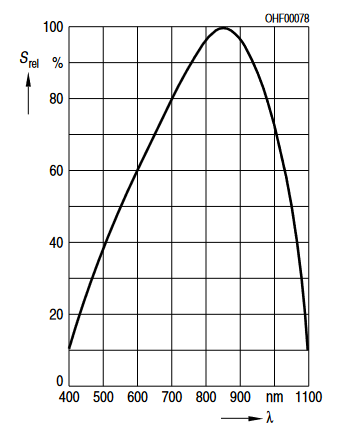
\includegraphics[width=\textwidth]{images/NewarkBPX61.png}
\end{figure}

\begin{figure}[H]
    \caption{NIR Photodiode Spectral Sensitivity}
    \centering
    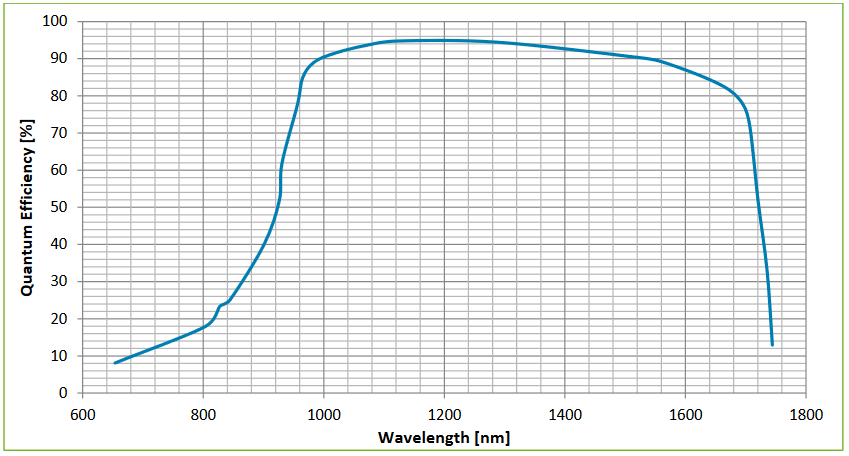
\includegraphics[width=\textwidth]{images/DigikeyExcilitasNIRSensor.png}
\end{figure}